\section{Recherche de la couleur de la voiture}
\begin{enumerate}
  \item \q{Faire afficher dans une même fenêtre externe l'image
          initiale en couleurs et les 3 images }\il{R}\q{, }\il{G}\q{ et }
        \il{B}\q{ en niveaux de rouge, vert bleu.}

        \codeFromFileT{helpers/image.py}{section-02/q1-1.py}
        \codeFromFileT{main.py}{section-02/q1-2.py}
        Ce qui donne : (j'ai éclaircit l'image pour l'impression)
        \begin{center}
          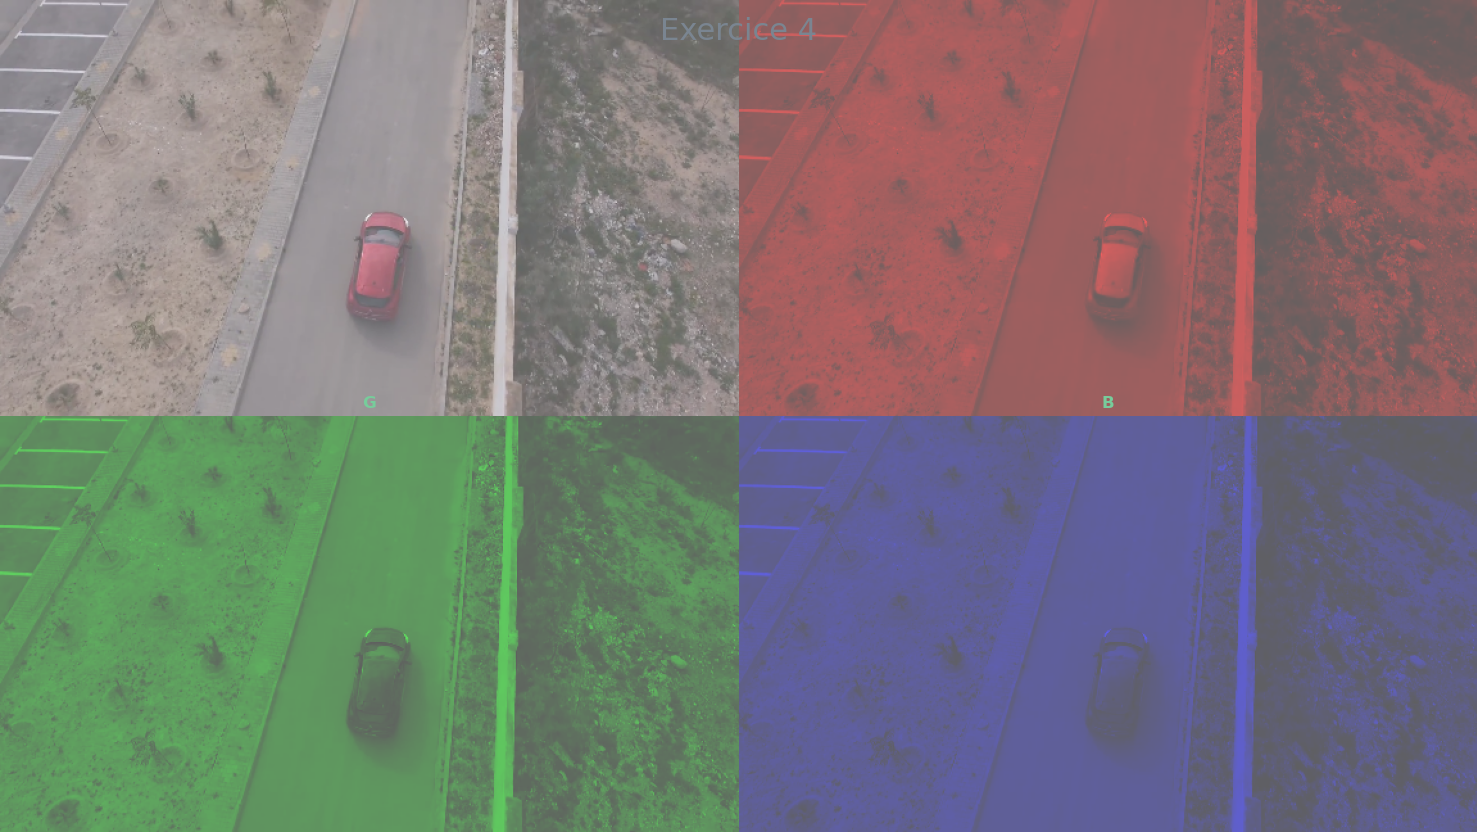
\includegraphics[scale=0.2]{section-02/q1-3.png}
        \end{center}
  \item \q{En faisant glisser la souris sur la voiture, on peut lire les niveaux
          de chaque couleur, en déduire 3 fourchettes approximatives dans
          lesquelles sont comprises les 3 couleurs R, G, B.}
        Je trouve :
        \[
          \left\{
          \begin{array}{rcl}
            R & = & 132 \\
            G & = & 25  \\
            B & = & 47  \\
          \end{array}
          \right.
        \]
\end{enumerate}
